\documentclass[twoside]{book}

% Packages required by doxygen
\usepackage{calc}
\usepackage{doxygen}
\usepackage{graphicx}
\usepackage[utf8]{inputenc}
\usepackage{makeidx}
\usepackage{multicol}
\usepackage{multirow}
\usepackage{textcomp}
\usepackage[table]{xcolor}

% Font selection
\usepackage[T1]{fontenc}
\usepackage{mathptmx}
\usepackage[scaled=.90]{helvet}
\usepackage{courier}
\usepackage{amssymb}
\usepackage{sectsty}
\renewcommand{\familydefault}{\sfdefault}
\allsectionsfont{%
  \fontseries{bc}\selectfont%
  \color{darkgray}%
}
\renewcommand{\DoxyLabelFont}{%
  \fontseries{bc}\selectfont%
  \color{darkgray}%
}

% Page & text layout
\usepackage{geometry}
\geometry{%
  a4paper,%
  top=2.5cm,%
  bottom=2.5cm,%
  left=2.5cm,%
  right=2.5cm%
}
\tolerance=750
\hfuzz=15pt
\hbadness=750
\setlength{\emergencystretch}{15pt}
\setlength{\parindent}{0cm}
\setlength{\parskip}{0.2cm}
\makeatletter
\renewcommand{\paragraph}{%
  \@startsection{paragraph}{4}{0ex}{-1.0ex}{1.0ex}{%
    \normalfont\normalsize\bfseries\SS@parafont%
  }%
}
\renewcommand{\subparagraph}{%
  \@startsection{subparagraph}{5}{0ex}{-1.0ex}{1.0ex}{%
    \normalfont\normalsize\bfseries\SS@subparafont%
  }%
}
\makeatother

% Headers & footers
\usepackage{fancyhdr}
\pagestyle{fancyplain}
\fancyhead[LE]{\fancyplain{}{\bfseries\thepage}}
\fancyhead[CE]{\fancyplain{}{}}
\fancyhead[RE]{\fancyplain{}{\bfseries\leftmark}}
\fancyhead[LO]{\fancyplain{}{\bfseries\rightmark}}
\fancyhead[CO]{\fancyplain{}{}}
\fancyhead[RO]{\fancyplain{}{\bfseries\thepage}}
\fancyfoot[LE]{\fancyplain{}{}}
\fancyfoot[CE]{\fancyplain{}{}}
\fancyfoot[RE]{\fancyplain{}{\bfseries\scriptsize Generated on Tue Jun 10 2014 19\-:15\-:53 for My Project by Doxygen }}
\fancyfoot[LO]{\fancyplain{}{\bfseries\scriptsize Generated on Tue Jun 10 2014 19\-:15\-:53 for My Project by Doxygen }}
\fancyfoot[CO]{\fancyplain{}{}}
\fancyfoot[RO]{\fancyplain{}{}}
\renewcommand{\footrulewidth}{0.4pt}
\renewcommand{\chaptermark}[1]{%
  \markboth{#1}{}%
}
\renewcommand{\sectionmark}[1]{%
  \markright{\thesection\ #1}%
}

% Indices & bibliography
\usepackage{natbib}
\usepackage[titles]{tocloft}
\setcounter{tocdepth}{3}
\setcounter{secnumdepth}{5}
\makeindex

% Hyperlinks (required, but should be loaded last)
\usepackage{ifpdf}
\ifpdf
  \usepackage[pdftex,pagebackref=true]{hyperref}
\else
  \usepackage[ps2pdf,pagebackref=true]{hyperref}
\fi
\hypersetup{%
  colorlinks=true,%
  linkcolor=blue,%
  citecolor=blue,%
  unicode%
}

% Custom commands
\newcommand{\clearemptydoublepage}{%
  \newpage{\pagestyle{empty}\cleardoublepage}%
}


%===== C O N T E N T S =====

\begin{document}

% Titlepage & ToC
\hypersetup{pageanchor=false}
\pagenumbering{roman}
\begin{titlepage}
\vspace*{7cm}
\begin{center}%
{\Large My Project }\\
\vspace*{1cm}
{\large Generated by Doxygen 1.8.5}\\
\vspace*{0.5cm}
{\small Tue Jun 10 2014 19:15:53}\\
\end{center}
\end{titlepage}
\clearemptydoublepage
\tableofcontents
\clearemptydoublepage
\pagenumbering{arabic}
\hypersetup{pageanchor=true}

%--- Begin generated contents ---
\chapter{Hierarchical Index}
\section{Class Hierarchy}
This inheritance list is sorted roughly, but not completely, alphabetically\-:\begin{DoxyCompactList}
\item \contentsline{section}{D}{\pageref{classD}}{}
\item \contentsline{section}{Documentation\-Check}{\pageref{classDocumentationCheck}}{}
\item \contentsline{section}{File\-Navigator}{\pageref{classFileNavigator}}{}
\begin{DoxyCompactList}
\item \contentsline{section}{C\-P\-P\-File\-Navigator}{\pageref{classCPPFileNavigator}}{}
\item \contentsline{section}{Scheme\-File\-Navigator}{\pageref{classSchemeFileNavigator}}{}
\end{DoxyCompactList}
\item \contentsline{section}{File\-Navigator\-Factory}{\pageref{classFileNavigatorFactory}}{}
\item \contentsline{section}{Node}{\pageref{classNode}}{}
\item \contentsline{section}{Tree}{\pageref{classTree}}{}
\end{DoxyCompactList}

\chapter{Class Index}
\section{Class List}
Here are the classes, structs, unions and interfaces with brief descriptions\-:\begin{DoxyCompactList}
\item\contentsline{section}{\hyperlink{classjudge__base}{judge\-\_\-base} }{\pageref{classjudge__base}}{}
\item\contentsline{section}{\hyperlink{classlocal__onlinejudge__renderer}{local\-\_\-onlinejudge\-\_\-renderer} }{\pageref{classlocal__onlinejudge__renderer}}{}
\item\contentsline{section}{\hyperlink{classonlinejudge__exception}{onlinejudge\-\_\-exception} }{\pageref{classonlinejudge__exception}}{}
\end{DoxyCompactList}

\chapter{Class Documentation}
\hypertarget{classCPPFileNavigator}{\section{C\-P\-P\-File\-Navigator Class Reference}
\label{classCPPFileNavigator}\index{C\-P\-P\-File\-Navigator@{C\-P\-P\-File\-Navigator}}
}
Inheritance diagram for C\-P\-P\-File\-Navigator\-:\begin{figure}[H]
\begin{center}
\leavevmode
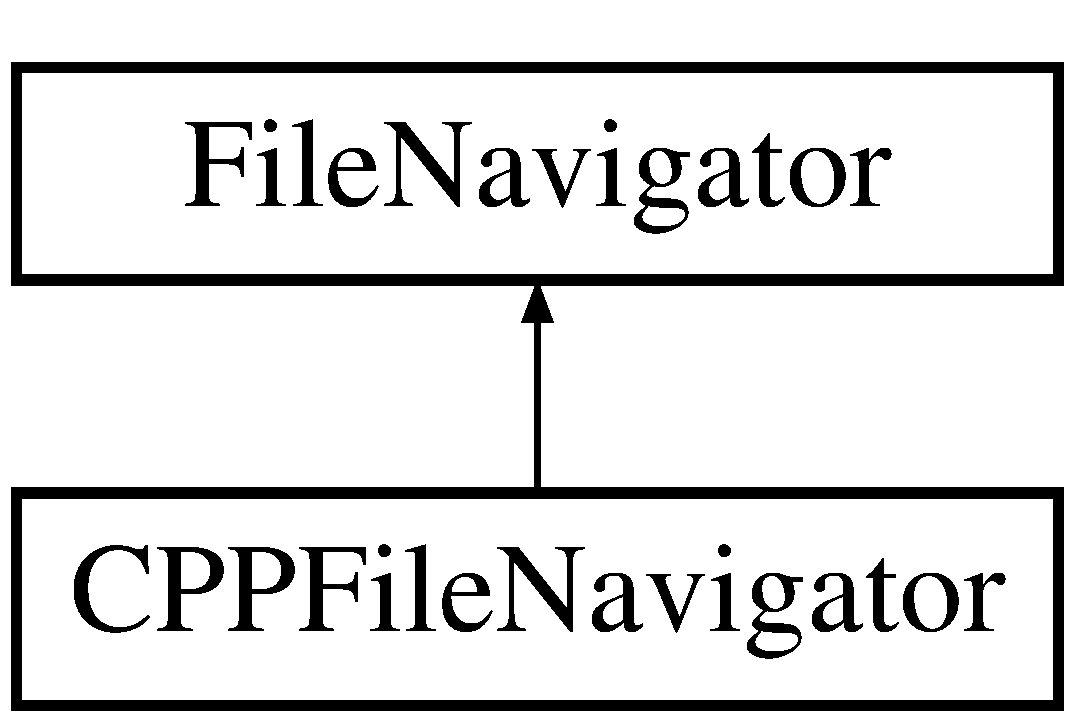
\includegraphics[height=2.000000cm]{classCPPFileNavigator}
\end{center}
\end{figure}
\subsection*{Additional Inherited Members}


\subsection{Detailed Description}
\begin{DoxyVersion}{Version}
0.\-1 
\end{DoxyVersion}
\begin{DoxyAuthor}{Author}
Oscar Chamat  \href{http://www.gnu.org/copyleft/gpl.html}{\tt http\-://www.\-gnu.\-org/copyleft/gpl.\-html} G\-N\-U G\-P\-L v3 or later
\end{DoxyAuthor}
Clase que realiza la lectura de un archivo con estructura de comentarios perteneciente a el lenguaje c++ 

The documentation for this class was generated from the following file\-:\begin{DoxyCompactItemize}
\item 
C\-P\-P\-File\-Navigator.\-java\end{DoxyCompactItemize}

\hypertarget{classD}{\section{D Class Reference}
\label{classD}\index{D@{D}}
}
\subsection*{Static Public Member Functions}
\begin{DoxyCompactItemize}
\item 
static void \hyperlink{classD_a1fdfd6621e5ae9cfea93043592fcb096}{dbg} (Object...\-o)
\end{DoxyCompactItemize}


\subsection{Detailed Description}
\begin{DoxyAuthor}{Author}
Oscar Chamat -\/civilian (\href{mailto:chamatoscar@gmail.com}{\tt chamatoscar@gmail.\-com}) 
\end{DoxyAuthor}
\begin{DoxyVersion}{Version}
0.\-3  \href{http://www.gnu.org/copyleft/gpl.html}{\tt http\-://www.\-gnu.\-org/copyleft/gpl.\-html} G\-N\-U G\-P\-L v3 or later
\end{DoxyVersion}
Pequeña clase que ayuda a debugear haciendo las lineas de debug más cortas y mas visibles 

\subsection{Member Function Documentation}
\hypertarget{classD_a1fdfd6621e5ae9cfea93043592fcb096}{\index{D@{D}!dbg@{dbg}}
\index{dbg@{dbg}!D@{D}}
\subsubsection[{dbg}]{\setlength{\rightskip}{0pt plus 5cm}static void D.\-dbg (
\begin{DoxyParamCaption}
\item[{Object...}]{o}
\end{DoxyParamCaption}
)\hspace{0.3cm}{\ttfamily [inline]}, {\ttfamily [static]}}}\label{classD_a1fdfd6621e5ae9cfea93043592fcb096}
Imprime el param o System.\-out.\-println(Arrays.\-deep\-To\-String(o)); 
\begin{DoxyParams}{Parameters}
{\em Objet} & ... o \\
\hline
\end{DoxyParams}


The documentation for this class was generated from the following file\-:\begin{DoxyCompactItemize}
\item 
D.\-java\end{DoxyCompactItemize}

\hypertarget{classDocumentationCheck}{\section{Documentation\-Check Class Reference}
\label{classDocumentationCheck}\index{Documentation\-Check@{Documentation\-Check}}
}
\subsection*{Public Member Functions}
\begin{DoxyCompactItemize}
\item 
\hyperlink{classDocumentationCheck_a1ae432e52b82ff95e64aa66898fadb72}{Documentation\-Check} (String\mbox{[}$\,$\mbox{]} args)  throws Exception 
\end{DoxyCompactItemize}
\subsection*{Static Public Member Functions}
\begin{DoxyCompactItemize}
\item 
static void \hyperlink{classDocumentationCheck_a8ccd6e628906e3c67aedc6e1c8927dc1}{main} (String\mbox{[}$\,$\mbox{]} args)  throws Exception 
\end{DoxyCompactItemize}


\subsection{Detailed Description}
\begin{DoxyVersion}{Version}
0.\-1 
\end{DoxyVersion}
\begin{DoxyAuthor}{Author}
Oscar Chamat  \href{http://www.gnu.org/copyleft/gpl.html}{\tt http\-://www.\-gnu.\-org/copyleft/gpl.\-html} G\-N\-U G\-P\-L v3 or later
\end{DoxyAuthor}
Script que califica en porcentajes dado como numeros entre 0 y 1 el promedio de cumplimiento de ciertas etiquetas de documentación en los diferentes archivos 

\subsection{Constructor \& Destructor Documentation}
\hypertarget{classDocumentationCheck_a1ae432e52b82ff95e64aa66898fadb72}{\index{Documentation\-Check@{Documentation\-Check}!Documentation\-Check@{Documentation\-Check}}
\index{Documentation\-Check@{Documentation\-Check}!DocumentationCheck@{Documentation\-Check}}
\subsubsection[{Documentation\-Check}]{\setlength{\rightskip}{0pt plus 5cm}Documentation\-Check.\-Documentation\-Check (
\begin{DoxyParamCaption}
\item[{String\mbox{[}$\,$\mbox{]}}]{args}
\end{DoxyParamCaption}
) throws Exception\hspace{0.3cm}{\ttfamily [inline]}}}\label{classDocumentationCheck_a1ae432e52b82ff95e64aa66898fadb72}
Constructor de la clase


\begin{DoxyParams}{Parameters}
{\em args} & parametros de configuracion \\
\hline
\end{DoxyParams}


\subsection{Member Function Documentation}
\hypertarget{classDocumentationCheck_a8ccd6e628906e3c67aedc6e1c8927dc1}{\index{Documentation\-Check@{Documentation\-Check}!main@{main}}
\index{main@{main}!DocumentationCheck@{Documentation\-Check}}
\subsubsection[{main}]{\setlength{\rightskip}{0pt plus 5cm}static void Documentation\-Check.\-main (
\begin{DoxyParamCaption}
\item[{String\mbox{[}$\,$\mbox{]}}]{args}
\end{DoxyParamCaption}
) throws Exception\hspace{0.3cm}{\ttfamily [inline]}, {\ttfamily [static]}}}\label{classDocumentationCheck_a8ccd6e628906e3c67aedc6e1c8927dc1}
main


\begin{DoxyParams}{Parameters}
{\em args} & parametros de configuracion \\
\hline
\end{DoxyParams}


The documentation for this class was generated from the following file\-:\begin{DoxyCompactItemize}
\item 
Documentation\-Check.\-java\end{DoxyCompactItemize}

\hypertarget{classFileNavigator}{\section{File\-Navigator Class Reference}
\label{classFileNavigator}\index{File\-Navigator@{File\-Navigator}}
}
Inheritance diagram for File\-Navigator\-:\begin{figure}[H]
\begin{center}
\leavevmode
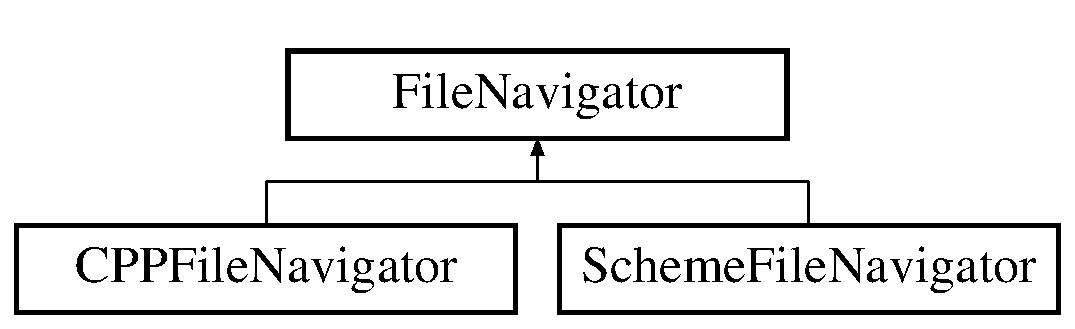
\includegraphics[height=2.000000cm]{classFileNavigator}
\end{center}
\end{figure}
\subsection*{Protected Attributes}
\begin{DoxyCompactItemize}
\item 
\hyperlink{classTree}{Tree} \hyperlink{classFileNavigator_a3db42b8bda212a686058434cceabe986}{t}
\end{DoxyCompactItemize}


\subsection{Detailed Description}
\begin{DoxyVersion}{Version}
0.\-1 
\end{DoxyVersion}
\begin{DoxyAuthor}{Author}
Oscar Chamat  \href{http://www.gnu.org/copyleft/gpl.html}{\tt http\-://www.\-gnu.\-org/copyleft/gpl.\-html} G\-N\-U G\-P\-L v3 or later
\end{DoxyAuthor}
Clase abstracta parte de un patron de diseño factory para poder navegar facilmente diferentes tipos de archivo 

\subsection{Member Data Documentation}
\hypertarget{classFileNavigator_a3db42b8bda212a686058434cceabe986}{\index{File\-Navigator@{File\-Navigator}!t@{t}}
\index{t@{t}!FileNavigator@{File\-Navigator}}
\subsubsection[{t}]{\setlength{\rightskip}{0pt plus 5cm}{\bf Tree} File\-Navigator.\-t\hspace{0.3cm}{\ttfamily [protected]}}}\label{classFileNavigator_a3db42b8bda212a686058434cceabe986}
Atributo que representa el arbol sintactico de un archivo. 

The documentation for this class was generated from the following file\-:\begin{DoxyCompactItemize}
\item 
File\-Navigator.\-java\end{DoxyCompactItemize}

\hypertarget{classFileNavigatorFactory}{\section{File\-Navigator\-Factory Class Reference}
\label{classFileNavigatorFactory}\index{File\-Navigator\-Factory@{File\-Navigator\-Factory}}
}
\subsection*{Static Public Member Functions}
\begin{DoxyCompactItemize}
\item 
static \hyperlink{classFileNavigator}{File\-Navigator} \hyperlink{classFileNavigatorFactory_ad719b3620140469db26eaf0effcb12f2}{get\-Instance} (String file, String lang)  throws I\-O\-Exception 
\end{DoxyCompactItemize}


\subsection{Detailed Description}
\begin{DoxyVersion}{Version}
0.\-1 
\end{DoxyVersion}
\begin{DoxyAuthor}{Author}
Oscar Chamat  \href{http://www.gnu.org/copyleft/gpl.html}{\tt http\-://www.\-gnu.\-org/copyleft/gpl.\-html} G\-N\-U G\-P\-L v3 or later
\end{DoxyAuthor}
Clase factoria parte de un patro de diseño factory para poder navegar facilmente diferentes tipos de archivo, crea un tipo de navegador dependiendo del lenguaje 

\subsection{Member Function Documentation}
\hypertarget{classFileNavigatorFactory_ad719b3620140469db26eaf0effcb12f2}{\index{File\-Navigator\-Factory@{File\-Navigator\-Factory}!get\-Instance@{get\-Instance}}
\index{get\-Instance@{get\-Instance}!FileNavigatorFactory@{File\-Navigator\-Factory}}
\subsubsection[{get\-Instance}]{\setlength{\rightskip}{0pt plus 5cm}static {\bf File\-Navigator} File\-Navigator\-Factory.\-get\-Instance (
\begin{DoxyParamCaption}
\item[{String}]{file, }
\item[{String}]{lang}
\end{DoxyParamCaption}
) throws I\-O\-Exception\hspace{0.3cm}{\ttfamily [inline]}, {\ttfamily [static]}}}\label{classFileNavigatorFactory_ad719b3620140469db26eaf0effcb12f2}
Retorna una instancia de \hyperlink{classFileNavigator}{File\-Navigator}


\begin{DoxyParams}{Parameters}
{\em } & \\
\hline
\end{DoxyParams}


The documentation for this class was generated from the following file\-:\begin{DoxyCompactItemize}
\item 
File\-Navigator\-Factory.\-java\end{DoxyCompactItemize}

\hypertarget{classNode}{\section{Node Class Reference}
\label{classNode}\index{Node@{Node}}
}
\subsection*{Public Member Functions}
\begin{DoxyCompactItemize}
\item 
\hyperlink{classNode_ac49d7bf2c7bab18b91c6c63fddfc5cb8}{Node} (String comment, int end\-Comment, int ini\-Comment)
\item 
\hyperlink{classNode_a36a5d1725e0943c7fbfe584ed4bd870d}{Node} (int ini\-Comment)
\item 
String \hyperlink{classNode_a5178447ba3e6a582f72c3b8bc217a78e}{to\-String} ()
\end{DoxyCompactItemize}


\subsection{Detailed Description}
\begin{DoxyVersion}{Version}
0.\-1 
\end{DoxyVersion}
\begin{DoxyAuthor}{Author}
Oscar Chamat  \href{http://www.gnu.org/copyleft/gpl.html}{\tt http\-://www.\-gnu.\-org/copyleft/gpl.\-html} G\-N\-U G\-P\-L v3 or later
\end{DoxyAuthor}
Clase que representa un nodo sintactico resultante de un analisis 

\subsection{Constructor \& Destructor Documentation}
\hypertarget{classNode_ac49d7bf2c7bab18b91c6c63fddfc5cb8}{\index{Node@{Node}!Node@{Node}}
\index{Node@{Node}!Node@{Node}}
\subsubsection[{Node}]{\setlength{\rightskip}{0pt plus 5cm}Node.\-Node (
\begin{DoxyParamCaption}
\item[{String}]{comment, }
\item[{int}]{end\-Comment, }
\item[{int}]{ini\-Comment}
\end{DoxyParamCaption}
)\hspace{0.3cm}{\ttfamily [inline]}}}\label{classNode_ac49d7bf2c7bab18b91c6c63fddfc5cb8}
Constructor de un nodo sintactico para la version 0.\-1 solo tiene en cuenta los comentarios, donde inician y donde finalizan 
\begin{DoxyParams}{Parameters}
{\em String} & comment el comentario de una o varias lineas \\
\hline
{\em int} & end\-Comment en que linea termina el comentario. \\
\hline
{\em int} & ini\-Comment en que linea inicia el comentario. \\
\hline
\end{DoxyParams}
\hypertarget{classNode_a36a5d1725e0943c7fbfe584ed4bd870d}{\index{Node@{Node}!Node@{Node}}
\index{Node@{Node}!Node@{Node}}
\subsubsection[{Node}]{\setlength{\rightskip}{0pt plus 5cm}Node.\-Node (
\begin{DoxyParamCaption}
\item[{int}]{ini\-Comment}
\end{DoxyParamCaption}
)\hspace{0.3cm}{\ttfamily [inline]}}}\label{classNode_a36a5d1725e0943c7fbfe584ed4bd870d}
Constructor de un nodo sintactico para la version 0.\-1 solo tiene en cuenta los comentarios, donde inician y donde finalizan 
\begin{DoxyParams}{Parameters}
{\em String} & comment el comentario de una o varias lineas \\
\hline
{\em int} & ini\-Comment en que linea inicia el comentario. \\
\hline
\end{DoxyParams}


\subsection{Member Function Documentation}
\hypertarget{classNode_a5178447ba3e6a582f72c3b8bc217a78e}{\index{Node@{Node}!to\-String@{to\-String}}
\index{to\-String@{to\-String}!Node@{Node}}
\subsubsection[{to\-String}]{\setlength{\rightskip}{0pt plus 5cm}String Node.\-to\-String (
\begin{DoxyParamCaption}
{}
\end{DoxyParamCaption}
)\hspace{0.3cm}{\ttfamily [inline]}}}\label{classNode_a5178447ba3e6a582f72c3b8bc217a78e}
Representación en string de el nodo actual \begin{DoxyReturn}{Returns}
String la representación. 
\end{DoxyReturn}


The documentation for this class was generated from the following file\-:\begin{DoxyCompactItemize}
\item 
Node.\-java\end{DoxyCompactItemize}

\hypertarget{classSchemeFileNavigator}{\section{Scheme\-File\-Navigator Class Reference}
\label{classSchemeFileNavigator}\index{Scheme\-File\-Navigator@{Scheme\-File\-Navigator}}
}
Inheritance diagram for Scheme\-File\-Navigator\-:\begin{figure}[H]
\begin{center}
\leavevmode
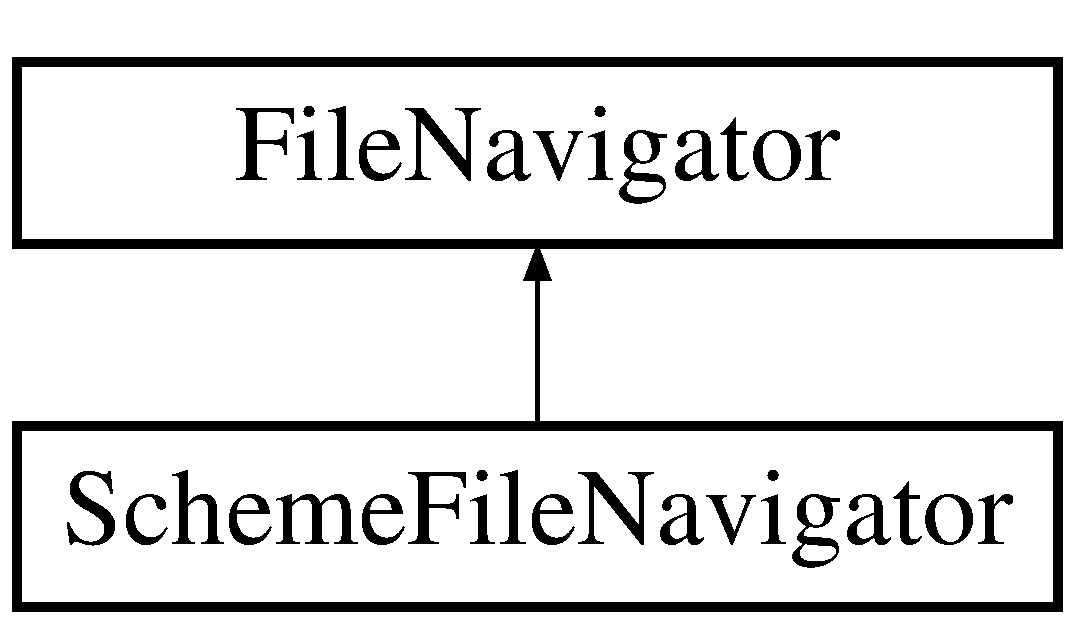
\includegraphics[height=2.000000cm]{classSchemeFileNavigator}
\end{center}
\end{figure}
\subsection*{Additional Inherited Members}


\subsection{Detailed Description}
\begin{DoxyVersion}{Version}
0.\-1 
\end{DoxyVersion}
\begin{DoxyAuthor}{Author}
Oscar Chamat  \href{http://www.gnu.org/copyleft/gpl.html}{\tt http\-://www.\-gnu.\-org/copyleft/gpl.\-html} G\-N\-U G\-P\-L v3 or later
\end{DoxyAuthor}
Clase que realiza la lectura de un archivo con estructura de comentarios perteneciente a el lenguaje dr\-Racket o dr\-Scheme 

The documentation for this class was generated from the following file\-:\begin{DoxyCompactItemize}
\item 
Scheme\-File\-Navigator.\-java\end{DoxyCompactItemize}

\hypertarget{classTree}{\section{Tree Class Reference}
\label{classTree}\index{Tree@{Tree}}
}
\subsection*{Public Member Functions}
\begin{DoxyCompactItemize}
\item 
\hyperlink{classTree_a207c06111ed2f0d99ab87d4a2e248f32}{Tree} ()
\item 
String \hyperlink{classTree_a7dc6e374b4f55cdc6f248dbc1642b4d7}{to\-String} ()
\item 
boolean \hyperlink{classTree_a919e156d8e953377644788787653b10f}{contains} (String string)
\end{DoxyCompactItemize}


\subsection{Detailed Description}
\begin{DoxyVersion}{Version}
0.\-1 
\end{DoxyVersion}
\begin{DoxyAuthor}{Author}
Oscar Chamat  \href{http://www.gnu.org/copyleft/gpl.html}{\tt http\-://www.\-gnu.\-org/copyleft/gpl.\-html} G\-N\-U G\-P\-L v3 or later
\end{DoxyAuthor}
Clase que representa el arbol sintactico resultante de un analisis 

\subsection{Constructor \& Destructor Documentation}
\hypertarget{classTree_a207c06111ed2f0d99ab87d4a2e248f32}{\index{Tree@{Tree}!Tree@{Tree}}
\index{Tree@{Tree}!Tree@{Tree}}
\subsubsection[{Tree}]{\setlength{\rightskip}{0pt plus 5cm}Tree.\-Tree (
\begin{DoxyParamCaption}
{}
\end{DoxyParamCaption}
)\hspace{0.3cm}{\ttfamily [inline]}}}\label{classTree_a207c06111ed2f0d99ab87d4a2e248f32}
Constructor de la clase incializa los nodos vacios del arbol 

\subsection{Member Function Documentation}
\hypertarget{classTree_a919e156d8e953377644788787653b10f}{\index{Tree@{Tree}!contains@{contains}}
\index{contains@{contains}!Tree@{Tree}}
\subsubsection[{contains}]{\setlength{\rightskip}{0pt plus 5cm}boolean Tree.\-contains (
\begin{DoxyParamCaption}
\item[{String}]{string}
\end{DoxyParamCaption}
)\hspace{0.3cm}{\ttfamily [inline]}}}\label{classTree_a919e156d8e953377644788787653b10f}
Chequea si una etiqueta de documentacion es utilizada en los nodos


\begin{DoxyParams}{Parameters}
{\em String} & string la etiqueta a ser chequeada\\
\hline
\end{DoxyParams}
\begin{DoxyReturn}{Returns}
true la etiqueta es utilizada; false no esta utilizada propiamente. 
\end{DoxyReturn}
\hypertarget{classTree_a7dc6e374b4f55cdc6f248dbc1642b4d7}{\index{Tree@{Tree}!to\-String@{to\-String}}
\index{to\-String@{to\-String}!Tree@{Tree}}
\subsubsection[{to\-String}]{\setlength{\rightskip}{0pt plus 5cm}String Tree.\-to\-String (
\begin{DoxyParamCaption}
{}
\end{DoxyParamCaption}
)\hspace{0.3cm}{\ttfamily [inline]}}}\label{classTree_a7dc6e374b4f55cdc6f248dbc1642b4d7}
Representación en string de el nodo actual

\begin{DoxyReturn}{Returns}
String la representación. 
\end{DoxyReturn}


The documentation for this class was generated from the following file\-:\begin{DoxyCompactItemize}
\item 
Tree.\-java\end{DoxyCompactItemize}

%--- End generated contents ---

% Index
\newpage
\phantomsection
\addcontentsline{toc}{part}{Index}
\printindex

\end{document}
